\chapter{Implementierung}
\section{Filter-Logik} \label{sec:implFilter}
\textbf{Ausgangssituation}

Der \gls{filter} ist der Teil der Programmlogik, der aus den \gls{rohdaten} die \gls{ergebnismenge} produziert. Dies geschieht anhand von durch den Nutzer gewählter \gls{filtervalue}e. Jeder dieser Werte ist einem übergeordneten \gls{attribut} zugeordnet.

Um zu filtern, wählt der Nutzer in der Benutzeroberfläche ein \gls{attribut} aus, zu dem er dann alle vorhandenen Werte angezeigt bekommt, die noch nicht zum Berechnen der \gls{ergebnismenge} genutzt werden. Daraufhin kann er einen oder mehrere Werte anwählen. Die Werte verschwinden aus der Werteliste und tauchen im gleichen Moment in der Sidebar am rechten Bildschirmrand, unter dem entsprechenden \gls{attribut} gruppiert, wieder auf. Diesen Vorgang kann der Nutzer für verschiedene \gls{attribut} wiederholen. Hat er einen falschen Wert übernommen, kann dieser durch einen Klick auf das Element in der Sidebar wieder entfernt werden und er \enquote{wandert} zurück in die dazugehörige Werteliste.
Derzeit ist der \gls{filter} additiv implementiert. Das bedeutet, es sind immer alle \gls{filter} in der \gls{ergebnismenge}, die einem der Kriterien entsprechen. In der Mengenlehre wäre das Äquivalent dazu die Vereinigungsmenge.

Das folgende Beispiel verdeutlicht die Filterfunktionalität für den ersten Anwendungsfall:

Auswahl des Nutzers:

\begin{itemize}
	\item Kontinent: Europa
	\item Klimazone: Tropische Klimazone
\end{itemize}

\begin{figure}[H]
 \centering
 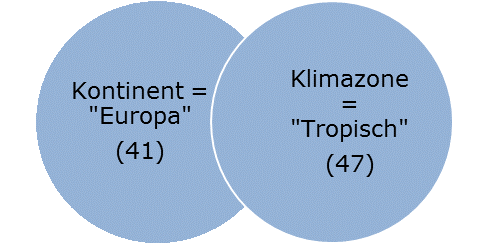
\includegraphics[width=0.5\textwidth]{grafiken/Filter_Vereinigung.png}
 \caption{Vereinigungsmenge Filter}
 \label{fig:filter1}
\end{figure}

Den Wert \enquote{Europa} unter dem \gls{attribut} Kontinent haben 41 Länder gesetzt, den Wert \enquote{Tropische Klimazone} unter dem \gls{attribut} \enquote{Klimazone}, 47 Länder. Die \gls{ergebnismenge} besteht nun aus allen Objekten, die mindestens eine der beiden Bedingungen erfüllen, also den 47 Objekten der Klimazonenbedingung und den 41 Ländern, die in Europa liegen. Natürlich werden die Werte, die beiden Bedingungen entsprechen nur einmal in der \gls{ergebnismenge} auftauchen (äquivalent zur Vereinigungsmenge). In diesem Beispiel käme man auf 84 Länder, die den Filtereinstellungen entsprechen.

\textbf{Problematik und Konzept}

Der \gls{filter} soll für die Anwendungsfälle 2 und 3 angepasst werden. Der Wunsch des Kunden ist eine Mischung aus dem additiven \gls{filter}, der bereits existiert, und einem \gls{filter}, bei dem die Filterauswahl die \gls{ergebnismenge} wieder einschränkt.

Die \gls{ergebnismenge} wird erweitert, wenn Werte des gleichen \gls{attribut}es ausgewählt werden. Die Einschränkung hingegen geschieht, wenn Werte eines anderen \gls{attribut}es ausgewählt werden.

Auch hier hilft die Mengenlehre, das Verhalten des \gls{filter}s zu verdeutlichen (Anwendungsfall 2):

Schritt 1 – Auswahl aus \gls{attribut} Motor:
\begin{itemize}
	\item Motor A
	\item Motor B
\end{itemize}

\begin{figure}[H]
 \centering
 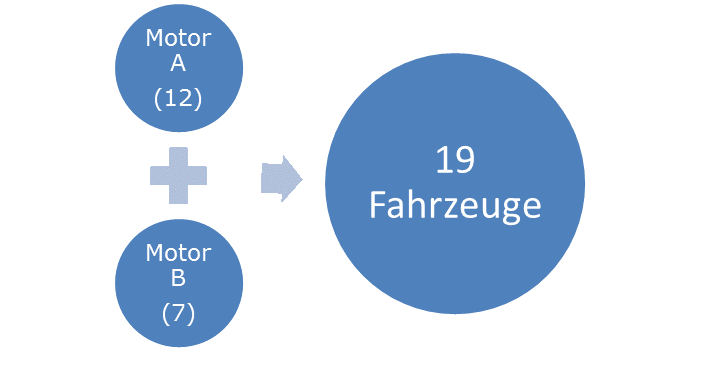
\includegraphics[width=0.7\textwidth]{grafiken/Filter_Motor.png}
 \caption{Teilmenge 1 - Exklusivfilter}
 \label{fig:filter2}
\end{figure}

Zu diesem Zeitpunkt besteht die \gls{ergebnismenge} aus genau diesen Fahrzeugen. Die Anzahl an Fahrzeugen der beiden Werte \enquote{Motor A} und \enquote{Motor B} können ohne weitere Bedenken addiert werden, da es keine Fahrzeuge mit 2 Motoren gibt.

Schritt 2 – Auswahl aus \gls{attribut} Getriebe
\begin{itemize}
	\item Getriebe A
	\item Getriebe B
\end{itemize}

\begin{figure}[H]
 \centering
 \includegraphics[width=0.7\textwidth]{grafiken/Filter_Getriebe.png}
 \caption{Teilmenge 2 - Exklusivfilter}
 \label{fig:filter3}
\end{figure}

Bei der Auswahl in Schritt 2 würden 15 Fahrzeuge in der \gls{ergebnismenge} landen. Da jetzt aber über zwei verschiedene \gls{attribut}e gefiltert wird, muss die \gls{ergebnismenge} aus den beiden einzelnen Ergebnissen berechnet werden. Dazu muss die Schnittmenge der beiden Teilmengen gebildet werden.

\begin{figure}[H]
 \centering
 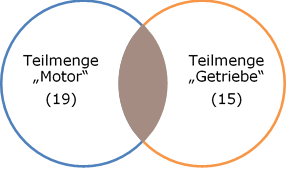
\includegraphics[width=0.5\textwidth]{grafiken/Filter_Schnitt.png}
 \caption{Schnittmenge - Exklusivfilter}
 \label{fig:filter4}
\end{figure}

Die \gls{ergebnismenge} ist in der Grafik genau der Bereich, in dem sich die beiden Teilmengen überschneiden. Sie enthält alle Elemente, die sowohl in der einen als auch in der anderen Teilmenge vorkommen.

Bei der Übernahme des Konzeptes auf die tatsächliche Implementierung des \gls{filter}s, muss allerdings bedacht werden, dass die Schnittmenge aus einer Vielzahl an \gls{attribut}en berechnet werden muss.

Zur Verbesserung der \gls{gebrauchstauglichkeit} des \gls{filter}s müssen in diesem Fall nach Selektion von Werten eines \gls{attribut}es die Wertelisten der anderen \gls{attribut}e aktualisiert werden, sodass durch die alleinige Auswahl von Werten verschiedener \gls{attribut}e kein leeres Ergebnis entstehen kann.

Im Umkehrschluss bedeutet das Vorhergegangene allerdings, dass die Wertelisten auch jedes Mal aktualisiert werden müssen, wenn ein Wert wieder aus der Filterselektion \enquote{rausgeworfen} wird. Dies muss auch geschehen, wenn sich dadurch eine gerade betrachtete Werteliste ändert.

\textbf{Umsetzung}

Auf technischer Seite ist der \gls{filter} so implementiert, dass es definierte Datenstrukturen für alle relevanten Mengen gibt. Folgende Strukturen existieren:

\begin{itemize}
	\item Menge aller \gls{filterattribut}e
	\item Alle Wertelisten, zugeordnet zu einem \gls{filterattribut}
	\item Zuordnung von Wertelisten mit (noch) selektierbaren Werten zu jeweils einem \gls{attribut}
	\item Menge aller \gls{filterattribut}e, von denen mindestens ein Wert selektiert wurde
	\item Zuordnung selektierter Werte zu einem \gls{filterattribut} aus zuvor genannter Menge
\end{itemize}

Um die obigen Mengen aktuell zu halten, also Änderungen in allen Mengen quasi-gleichzeitig zu publizieren werden \gls{javafx}-Listener benutzt. Wird die Menge der selektierten Werte geändert, werden die anderen Mengen aktualisiert.

Der \gls{filter} wird durch einen \gls{dataProvider} und durch einen FilterDataProvider gestützt. Der \gls{dataProvider} liefert alle existierenden Modellobjekte, die behandelt werden sollen und der FilterDataProvider stellt die \gls{attribut}e sowie die verfügbaren Werte zur Verfügung.

Die Logik führt bisher die in dem Abschnitt Ausgangssituation beschriebenen Mengenoperation mit einigen Besonderheiten aus. So gibt es zum Beispiel unterschiedliche Attributtypen. Es gibt \textit{ValueListFilterAttributes}, die die oben genannten Wertelisten beinhalten, \textit{BooleanFilterAttributes}, die nur die Werte Ja und Nein beinhalten und es gibt \textit{ParentFilterAttributes}, die dazu dienen, andere \gls{filterattribut}e zu gruppieren und diese \gls{filterattribut}e als Sublisten der ParentFilterAttribute darzustellen. Um die Beschreibung der Änderungen auf das Wesentliche zu reduzieren, wird auf diese und weitere Eigenheiten nicht näher eingegangen.

Die Änderungen am Quellcode umfassen im Groben folgendes:

Für die Methode \textit{\#isInFilter(Modelobjekt)}, die überprüft, ob ein Objekt den gewählten Filterkriterien entspricht, wurde eine Fallunterscheidung eingeführt. Diese erlaubt es, dass der \gls{filter} für den Anwendungsfall 1 wie bisher funktioniert, für den 2. Anwendungsfall jedoch das Schnittmengenkonzept implementiert. Dazu wird für jedes selektierte \gls{attribut} überprüft, ob der Wert, den das Modelobjekt für das entsprechende \gls{attribut} gesetzt hat, in der Menge der selektierten Werte vorhanden ist. Ist dies für ein \gls{attribut} nicht der Fall, bedeutet das, das geprüfte Modelobjekt darf nicht in der \gls{ergebnismenge} vorhanden sein.

Auch die Wertelisten mit den auswählbaren Werten aktualisieren sich jetzt zeitgleich mit der Filterselektion. Dies erforderte mehr Aufwand, da die Wertelisten nach Definition nur durch die Selektion von Werten eingeschränkt werden dürfen, die einem anderen \gls{attribut} zugeordnet sind als die betrachtete Werteliste. Um dies zu realisieren wurde eine neue Menge zu den oben beschriebenen Mengen hinzugefügt, die parallel zu den selektierbaren Werten eine gefilterte Sicht auf diese Werte bietet. Um die einzelnen Listen zu erzeugen, die jeweils einem \gls{attribut} zugeordnet sind, benötigt es zum einen eine Änderung an der \textit{\#isInFilter(Modelobjekt)} Methode und zum Anderen die Aktualisierung bei Änderung der selektierten Werte. Bei der \textit{\#isInFilter(Modelobjekt)} Methode kam ein neuer Parameter hinzu, welcher ein zu ignorierendes \gls{attribut} entgegennimmt. Das \enquote{Exklusiv-Attribut} wird dann bei der darauf folgenden Berechnung nicht mit einbezogen.

\begin{lstlisting}[
    language=Java,
    caption=Auszug aus Code der Methode \textit{\#isInFilter(Modelobjekt\, Filterattribut)},
    label=code9]
	[...]
	for (AbstractFilterAttribute<A> attribute : selectedAttributes) {
		if (!attribute.equals(exclusiveAttribute)) {
			Object attributeValue = dataProvider.resolve(dataObject, attribute.getAttributeName());
			if (!isValueSelected(attribute, value)) {
					return false;
			}
    	}
	}
	return !selectedValues.isEmpty();
	// returns true when loop passed through and false when there is no selection
	[...]
\end{lstlisting}

Diese Berechnung wird für jedes Modelobjekt ausgeführt um festzustellen, ob es in der \gls{ergebnismenge} inbegriffen ist, oder nicht. Die einzelnen, den \gls{attribut}en zugeordneten, Wertelisten der nicht-selektierten \gls{filtervalue}e, begründen sich gemäß der Implementierung auf der Berechnung einer Pseudo-\gls{ergebnismenge}, die das \gls{attribut} der betrachteten Werteliste nicht berücksichtigt. Die Attributwerte aller übrig gebliebenen Modelobjekte, die nicht in der Pseudo-\gls{ergebnismenge} vorhanden sind, dienen dazu, die spezielle Werteliste zu befüllen. So wird vermieden, dass \gls{filtervalue}e angewählt werden, die zu einer leeren \gls{ergebnismenge} führten.

Andersherum betrachtet ist es nicht so einfach möglich, zu verhindern, dass durch das \enquote{rauswerfen} von Attributwerten aus der Filterselektion, eine leere \gls{ergebnismenge} geschaffen wird. Um dies zu realisieren, müsste die Handlungsfreiheit des Nutzers stark eingeschränkt werden und verhindert werden, dass solche Attributwerte deselektiert werden. Zudem erforderte dies eine ständige Neuberechnung der möglichen \gls{ergebnismenge}, falls ein bestimmter Wert aus der Filterauswahl \enquote{geworfen} werden würde – und dies für jeden möglichen Wert, der entfernt werden kann.

\section{DataProvider} \label{sec:implDataProvider}
\textbf{Struktur}

Der \gls{dataProvider} versorgt, wie der Name schon andeutet, die einzelnen Bereiche der Anwendungslogik mit Daten aus dem Model. Es gibt für jeden Anwendungsfall einen eigenen \gls{dataProvider}, da jedes Szenario auf einer eigenen Art von Modelobjekten beruht. Die Klasse stellt neben den Modellobjekten weitere Methoden zum Auflösen von Attributwerten bereit. Dazu nimmt die Methode ein Modellobjekt und ein \gls{attribut} entgegen und liefert den dazugehörigen Wert zurück.

\begin{figure}[H]
 \centering
 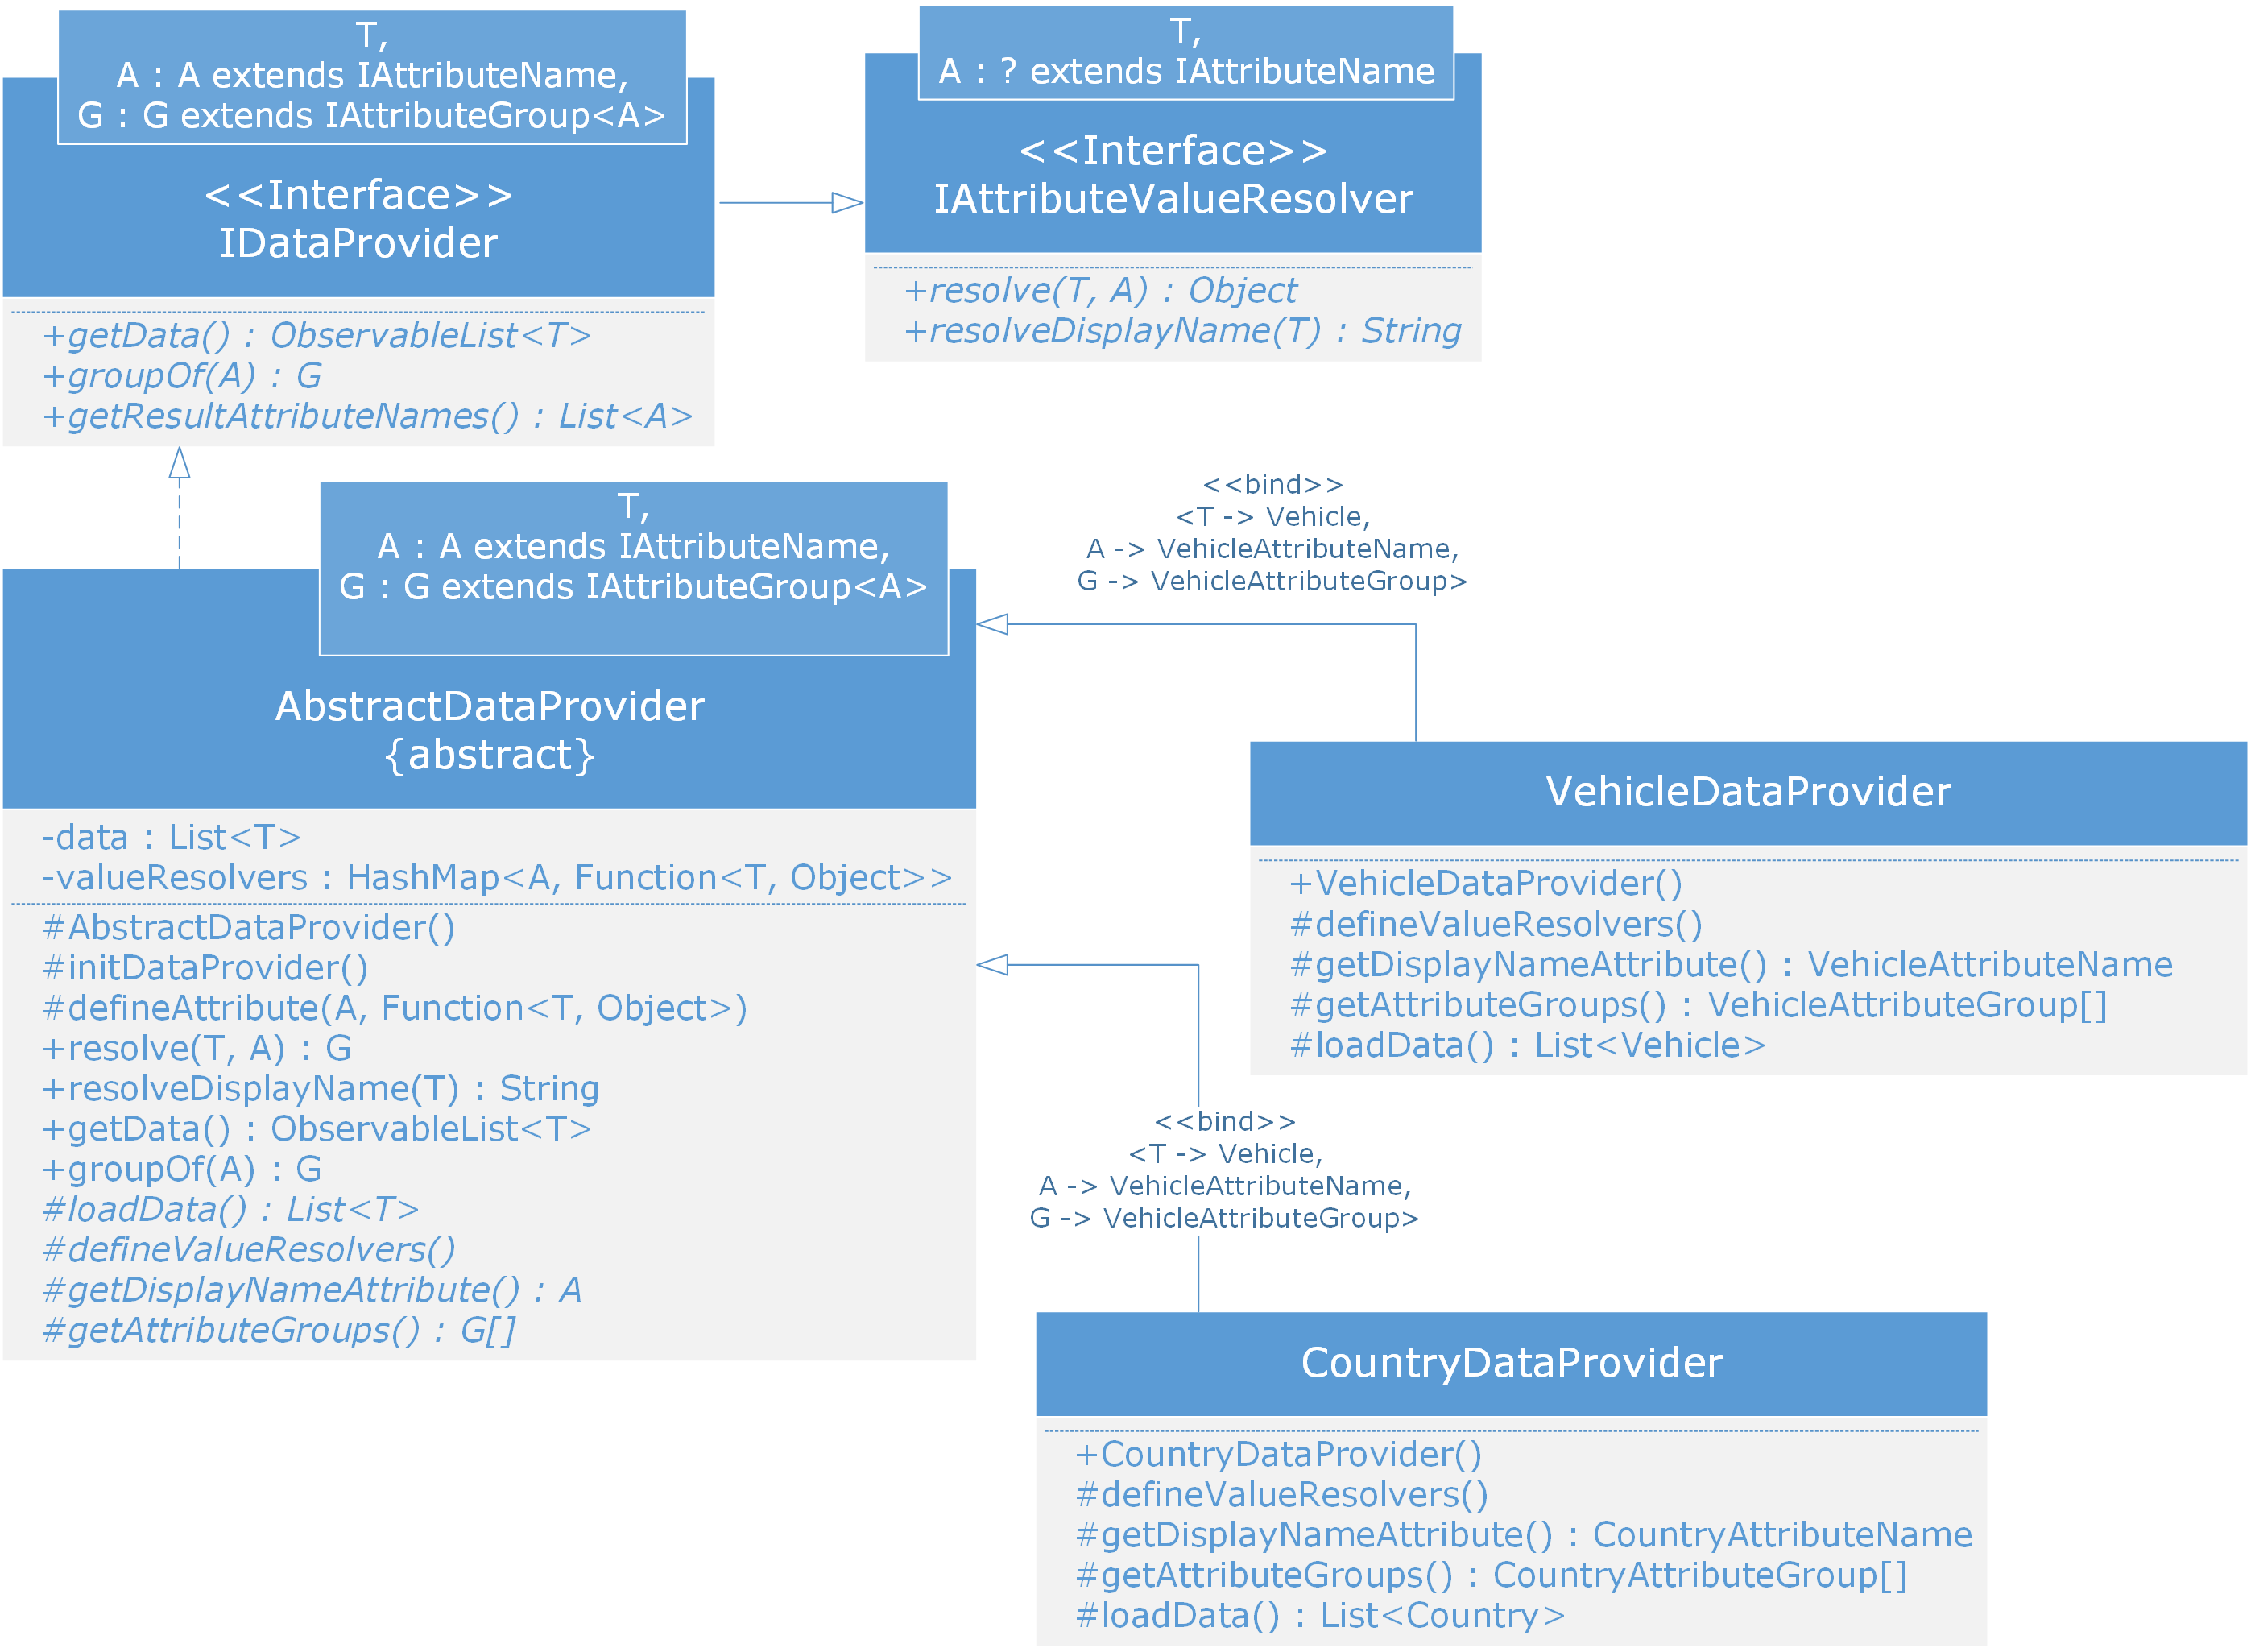
\includegraphics[width=1\textwidth]{grafiken/Class_DataProvider.png}
 \caption{Klassendiagramm DataProvider}
 \label{fig:dataProvider1}
\end{figure}

Die bestehende Klassenstruktur enthält bereits Interfaces und abstrakte Klassen, welche die Implementierungsstruktur eines \gls{dataProvider}s vorgeben. Die Grafik \ref{fig:dataProvider1} zeigt einen Ausschnitt der Klassenhierarchie und stellt die zum Verständnis relevanten Member dieser Klassen dar. Das hierarchisch höchste Interface \textit{IAttribute\gls{valueResolver}} liefert Funktionen, die für das Auflösen spezieller Werte zuständig sind. Anhand eines Modelobjektes T, mit dem das Interface als generischer Parameter wurde, und einem \gls{attribut}, das das Interface \textit{IAttributeName} implementieren muss, kann ein Wert erhalten werden (z.B. \enquote{Spanien} für das \gls{attribut} Land).
Ein weiteres Interface stellt der \textit{I\gls{dataProvider}} dar, der von \textit{IAttribute\gls{valueResolver}} ableitet. Hier werden Methoden definiert, um die Modelobjekte dieses \gls{dataProvider}s zu erhalten. Außerdem kann man per Methodenaufruf die \gls{attribut}e bekommen, die für die Ergebnisanzeige benötigt werden und die Zuordnung eines \gls{attribut}es zu einer Attributgruppe.

Der \textit{AbstractDataProvider} bietet nun die ersten Implementierungen für die abstrakten Methoden der Interfaces an. Zusätzlich werden weitere abstrakte Methoden hinzugefügt, die die konkrete Implementierung durch Unterklassen erfordern. Die Methoden werden für das Laden der Daten aus der Datenbank, sowie der Definition von \gls{valueResolver}s  benötigt. Ein \gls{valueResolver} beschreibt mithilfe einer Java8-\textit{Function}, wie für ein bestimmtes \gls{attribut} bei Eingabe eines Modelobjektes T, der Wert für dieses \gls{attribut}erhalten werden kann. Ein Resolver ist immer genau einem \gls{attribut} zugeordnet - und umgekehrt.

\textbf{Problemstellung}

Es soll parallel zu dem \textit{CountryDataProvider} und dem \textit{VehicleDataProvider} der \gls{dataProvider} für den 3. Anwendungsfall implementiert werden. Dazu gehört die Definition der \gls{attribut}e, die durch das Interface IAttribute\gls{valueResolver} benötigt werden, mit der jeweiligen Zuordnung zu einer Attributgruppe. Zusätzlich muss eine Datenstruktur entwickelt werden, die die geladenen Informationen in einem Objekt zusammenfasst – also die kombinierten Länder und Fahrzeugdaten zusammen mit den Produktionsfreigaben.

\textbf{Umsetzung}

Zunächst müssen die \gls{attribut}e definiert werden. Diese sind abhängig von der Ergebnispräsentation. Gemäß Anforderung sollen in der Ergebnistabelle Details zu den Fahrzeugen angezeigt werden und die Start/ Enddaten der Produktionsfreigaben. Daher entsprechen die definierten \gls{attribut}e in erster Linie den \gls{attribut}en aus dem Fahrzeug-Szenario. Aus diesem Grund müssen die \gls{attribut}e nicht alle neu definiert werden, sondern können durch eine statische Methode \textit{\#createAttributeName(IAttributeName)} erzeugt werden. Das neu erzeugte \gls{attribut} dient nur als Kapselung für das eigentliche \gls{attribut}, welches aus der Menge der Fahrzeug-Attribute kommt. Die Methode wird für jedes Fahrzeug-Attribut durch die bei der Definition der Attributgruppen aufgerufen. In dem Enum der Attributgruppen werden dem Konstruktor die Original-Attributgruppen übergeben und die \gls{attribut}e für den 3. Anwendungsfall können per Iteration über die zugeordneten Attributnamen erzeugt werden. Um zu vermeiden, dass \gls{attribut}e mehrfach definiert werden, werden die gekapselten \gls{attribut}e in einer statischen \textit{Map} gespeichert, die als \textit{Key} das Original-\gls{attribut} enthält und als Value den Wrapper zur Verfügung stellt. Zusätzlich zu den Wrapper-Attributen gibt es statische \gls{attribut}e, die für die Produktionsfreigabedaten stehen.

Im \gls{dataProvider} müssen, nachdem die \gls{attribut}e erzeugt wurden, die \gls{valueResolver}s beschrieben werden. Es muss also für jeden Attributnamen eine \textit{Function} implementiert werden. Allerdings kann, durch überschreiben der \textit{\#resolve(Modelobjekt, AttributeName)}-Methode doppelter Code vermieden werden. Wie bereits erläutert, stammen viele der \gls{attribut}e aus dem Fahrzeug-Anwendungsfall und so kann der Original-\gls{dataProvider} genutzt werden, um die Werte für die meisten \gls{attribut}e aufzulösen. Es müssen nur noch die Resolver für die hinzugekommenen \gls{attribut}e definiert werden.

In der Theorie werden für den 3. Anwendungsfall die Daten aus dem Länder-An\-wen\-dungs\-fall mit den Daten aus dem Fahrzeug-Anwendungsfall kombiniert und mit zusätzlichen Daten, den Produktionsfreigaben versehen. Dies geschieht für jede Kombination aus Fahrzeugen und Ländern, für die es eine Produktionsfreigabe gibt. Da die Menge an Produktionsfreigaben mit allen daran registrierten Daten lange Ladezeiten und sehr viel Speicher erfordern würde, können die Produktionsfreigaben vorab nicht geladen werden. Stattdessen werden, um Werte für den \gls{filter} bereitzustellen, zunächst nur die Länder- und die Fahrzeugdaten aus der Datenbank geladen. Gekapselt werden diese Daten in einer Datenstruktur \gls{filterElement}. Diese Struktur wird im nächsten Kapitel genauer erläutert.

\section{Multi-Filter} \label{sec:implMulti-Filter}
\textbf{Problemstellung}

Für den neuen Anwendungsfall ändern sich nun auch die Anforderungen an den \gls{filter}. Die Auswahl beruhte bislang nur auf Modellobjekten, die fachlich genau eine Art von anzuzeigenden Daten repräsentierten. Die Länderobjekte stellten Länder mit gewissen Eigenschaften dar und die Fahrzeugobjekte standen für Fahrzeuge. Die Modellobjekte für die neuen Funktionen hingegen bestehen nach dem Laden der Daten aus 2 verschiedenen Datensätzen (Land und Fahrzeug) und zur Zeit der Anzeige sogar aus 3 Datensätzen (zusätzlich die Produktionsfreigabe-Objekte).

Die \gls{ergebnismenge}, die auf dem \gls{filter} basiert, soll frei konfigurierbar sein. Das bedeutet, es sollen Produktionsfreigaben für eine beliebige Kombination von Ländern mit Fahrzeugen angezeigt werden können. Um das zu ermöglichen werden zwei voneinander unabhängig konfigurierbare \gls{filter} benötigt, die im Endeffekt jedoch zu einer einzelnen \gls{ergebnismenge} führen. Die einzelnen \gls{filter} sollen analog zu ihren jeweiligen ursprünglichen Anwendungsfällen implementiert werden. Der Länderfilter soll additiv funktionieren (siehe Abschnitt \ref{sec:implFilter} - Ausgangssituation) und der Fahrzeug-Filter einschränkend (siehe Abschnitt \ref{sec:implFilter} - Problematik und Konzept).

Nach der Auswahl der \gls{filtervalue}e müssen die Produktionsfreigaben in die Land-\-Fahr\-zeug-Kom\-bi\-na\-tio\-nen eingefügt werden.

\textbf{Umsetzung}

Die erste Problematik bezieht sich darauf, wie ein solcher \gls{filter} umzusetzen ist. Eine Möglichkeit wäre es, die Klasse \gls{filter} dahingehend umzuschreiben, dass sie sowohl mit einem als auch mit 2 Modellobjekten arbeiten kann. Der Vorteil dieser Lösung läge vor Allem darin, dass nur wenige Klassen bearbeitet werden müssten.
Eine andere Möglichkeit ist, die Filterlogik zu belassen und stattdessen die umgebende Struktur so zu verändern, dass 2 Instanzen des \gls{filter}s gleichzeitig und unabhängig voneinander verwendet werden können.

Da die Logik der \gls{filter}-Klasse mit verschiedenen Sonderbehandlungen ohnehin schon recht komplex ist, ist die zweite Möglichkeit in diesem Falle zu bevorzugen.
Folgend ist die Methodenschnittstelle der \gls{filter}-Klasse aufgeführt.

\begin{figure}[H]
 \centering
 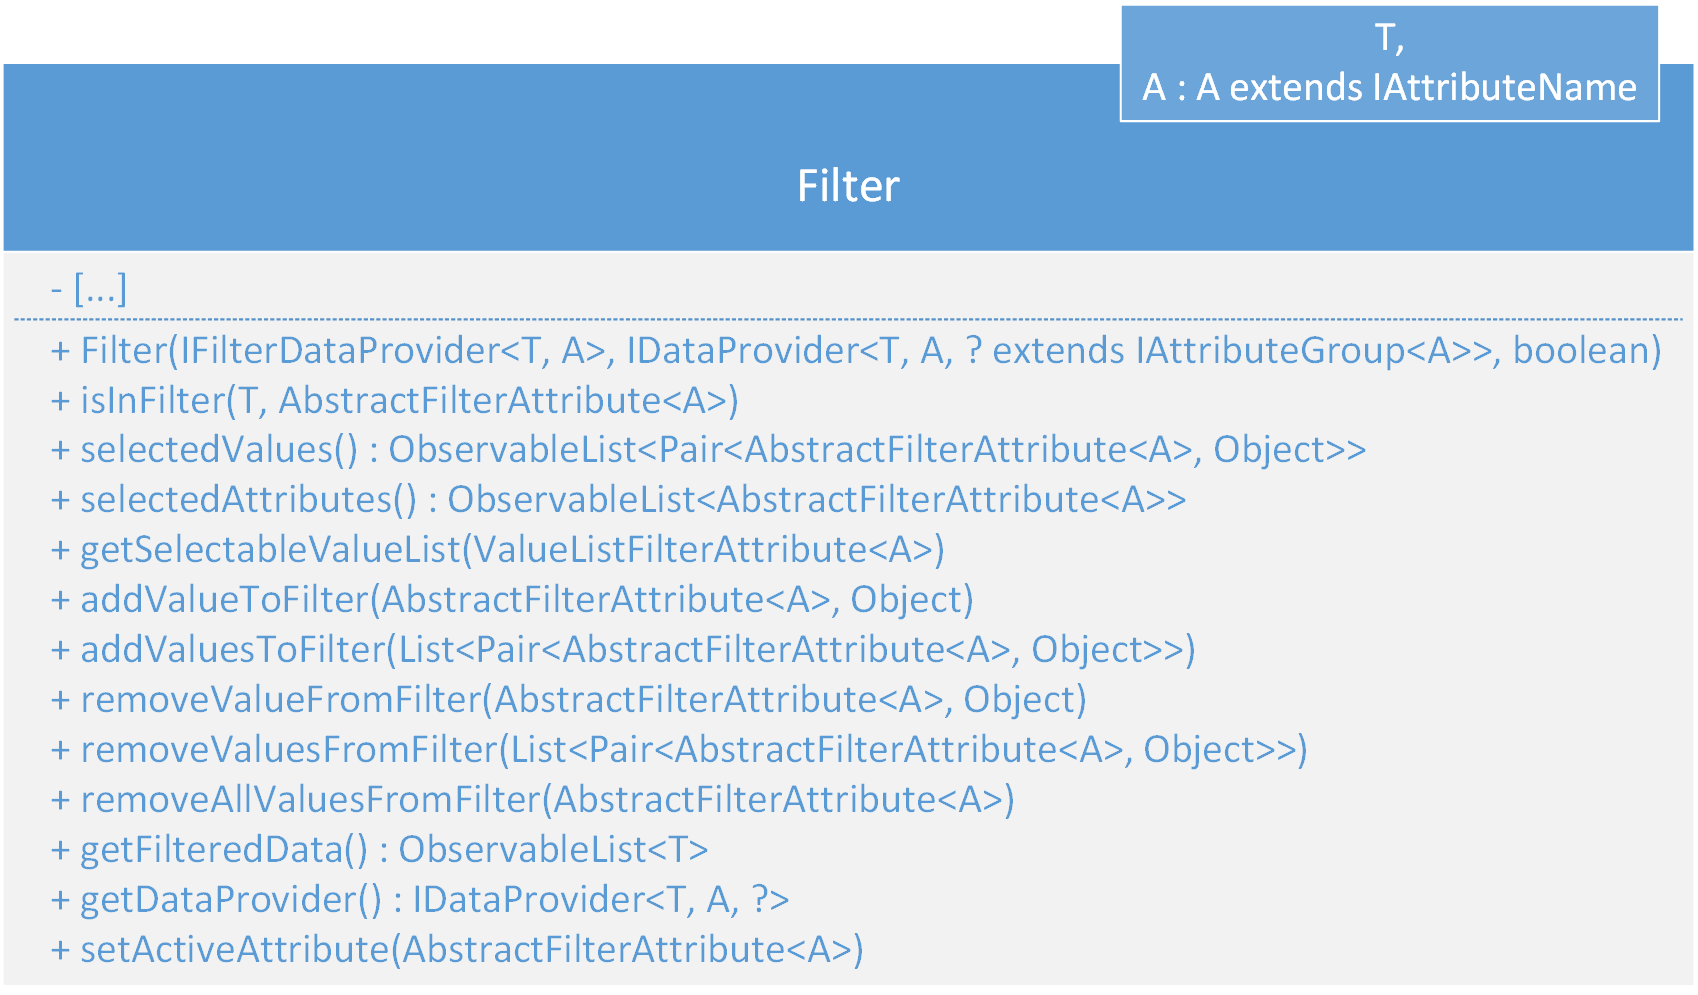
\includegraphics[width=0.85\textwidth]{grafiken/Class_Filter.png}
 \caption{Klassenaufbau - Filter}
 \label{fig:multiFilter1}
\end{figure}

Die Schnittstelle bietet Methoden, um auf die in Abschnitt \ref{sec:implFilter} - Umsetzung definierten Mengen zuzugreifen. Es zeigt sich, dass einige Mengen  nicht ganz wie erwartet implementiert sind. Im Beispiel der \textit{selectedValues} wird eine \textit{ObservableList} (\gls{javafx}) vom Typ \textit{Pair<AbstractFilterAttribute<A>, Object>} verwendet, anstatt der naheliegenden \textit{Map} mit der Typisierung \textit{<AbstractFilterAttribute<A>, List<Object>>}. Diese Entscheidung wurde getroffen, da sonst eine Benachrichtigung per \gls{javafx}-Listener über eine Änderung an dieser Menge nur auf umständlichem Wege möglich wäre. Dies ist bei mehreren dieser Mengen der Fall.

Eine weitere Auffälligkeit ist die häufige Verwendung von Generics. Wie bereits zuvor erwähnt, verarbeitet der \gls{filter} verschiedene Arten von Modellobjekten. Um dies zu bewerkstelligen, benötigt er nur die Informationen aus dem bereits erläuterten \gls{dataProvider} und weitere Information aus einem FilterDataProvider. Neben dem \gls{filter} gibt es noch viele weitere Klassen, die generisch implementiert sind.

Für den FilterDataProvider gibt es ebenfalls pro Anwendungsfall eine spezifische Implementierung. Für die Aufgabe ist dieser Teil der Logik jedoch nur bedingt relevant. Im Wesentlichen erstellt der FilterDataProvider aus den Modellobjekten des spezifischen Szenarios die Wertelisten für jedes \gls{attribut} zusammen indem er alle Modellobjekte durchläuft, die verschiedenen Werte zusammenträgt und gleiche Elemente zu einem zusammenfasst.

Um die Filteranforderungen umzusetzen muss nun eine Klasse geschrieben werden, die zwei dieser \gls{filter} verwaltet und Methodenaufrufe entsprechend delegiert. Dies kann wieder auf verschiedene Arten geschehen. Eine Möglichkeit wäre es, eine Art Provider für den \gls{filter} zu entwerfen. An diesem müssten dann Verwendungsstellen den \gls{filter} abfragen und würden, je nach Status der Anwendung, den Länder- oder den Fahrzeugfilter zurückbekommen. Da viele Verwendungsstellen den \gls{filter} jedoch zwischenspeichern und mit dem Umbau auf eine Providerstruktur auch gleichzeitig die Verwendung eines einzelnen \gls{filter}s (Anwendungsfall 1 und 2) komplizierter werden würde, ist diese Lösung eher ungeeignet.

Als Alternative dazu kann man einen neuen \gls{filter} entwerfen, der die anderen beiden \gls{filter} verwaltet. Für die Realisierung muss als Erstes der bestehende \gls{filter} abstrahiert werden. Sämtliche Methoden der Schnittstelle des \gls{filter}s müssen in die Oberklasse verschoben werden. Für diesen Fall bietet es sich an eine Abstrakte Klasse zu konstruieren, von der der bestehende \gls{filter} ableitet und die public Methoden der Schnittstelle überschreibt. Diese neue Klasse wird \textit{AbstractFilter} genannt und bekommt dieselben generischen Typen zugewiesen wie die Klasse \gls{filter}. In den Verwendungsstellen muss nur (außer bei dem Konstruktoraufruf) \enquote{Filter} durch \enquote{AbstractFilter} ersetzt werden und das Programm funktioniert genauso wie zuvor. Für die neue Funktionalität wird eine weitere Klasse eingeführt, die ebenfalls von dem AbstractFilter ableitet und zwei konkrete Instanzen der \gls{filter}-Klasse (Länder- und Fahrzeugfilter) verwaltet.

\begin{figure}[H]
 \centering
 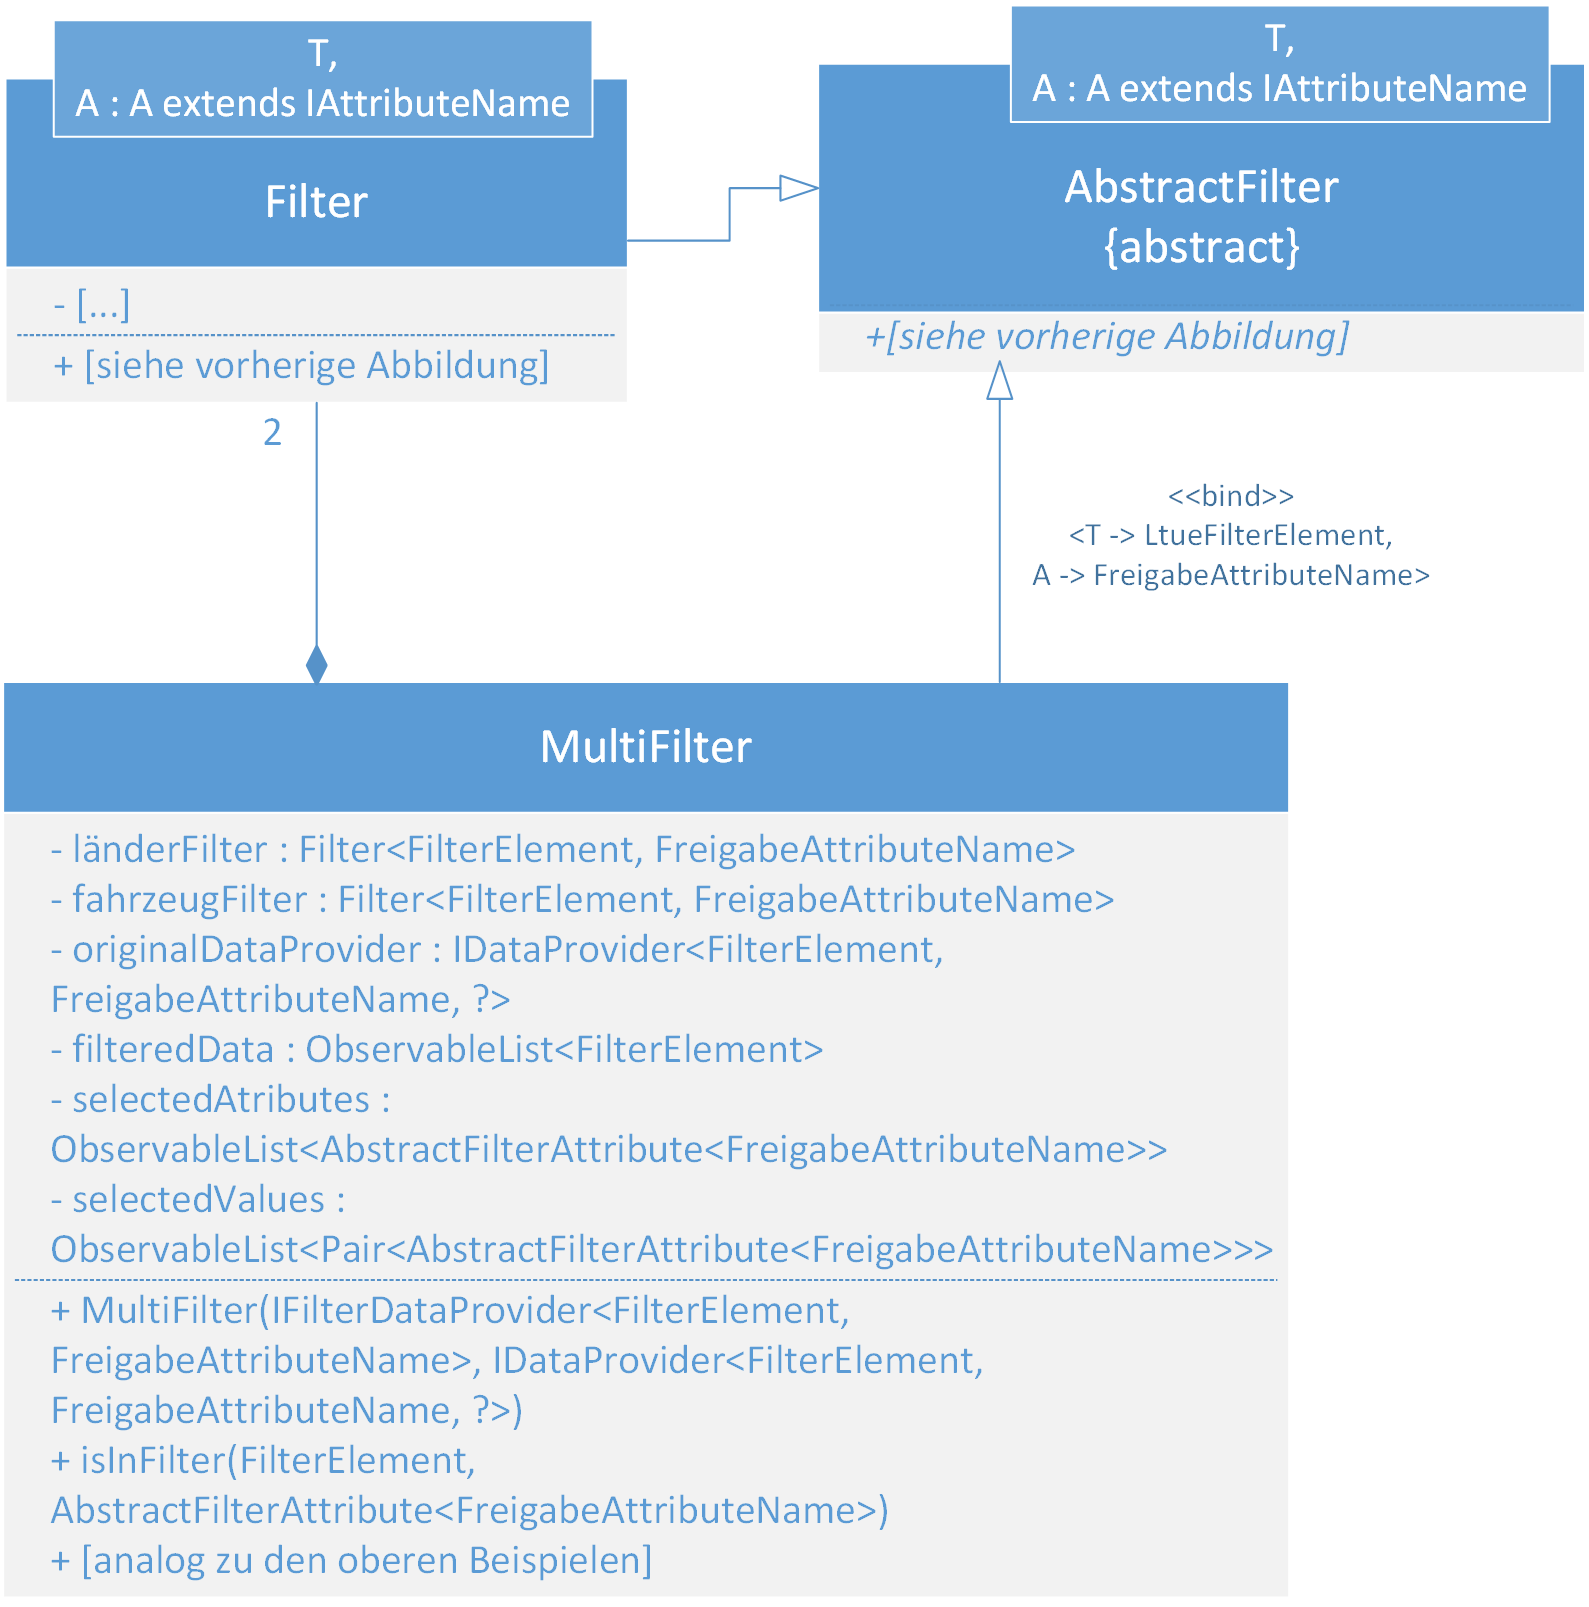
\includegraphics[width=0.85\textwidth]{grafiken/Class_MultiFilter.png}
 \caption{Klassendiagramm - Konzept Filter}
 \label{fig:multiFilter2}
\end{figure}

In der Abbildung \ref{fig:multiFilter2} sind die neuen Beziehungen zwischen den Filter-Klassen visualisiert. Um diese Struktur verwenden zu können, muss im 3. Anwendungsfall, statt eines normalen \gls{filter}s, der neue \gls{multiFilter} initialisiert werden. Wie dem Entwurf der \textit{MulitFilter}-Klasse (Abb. \ref{fig:multiFilter2}) entnommen werden kann, erwartet der \gls{multiFilter} als Modelobjekte die \gls{filterElement}e. Diese sind dreiteilig aufgebaut.

\begin{enumerate}
	\item Der Länderteil
	\item Der Fahrzeugteil
	\item Der Freigabeteil
\end{enumerate}

Mit \gls{getter}n und \gls{setter}n kann auf diese zugegriffen werden. Die Problematik besteht an dieser Stelle zunächst darin, ein \gls{filterElement} einem der zwei Sub-Filter zuzuordnen. Dies wird realisiert, indem die \gls{filterElement}e, die in einer einzelnen Liste vom \gls{dataProvider} zur Verfügung gestellt werden, verschiedene Ausprägungen besitzen. Wie in Kapitel \ref{sec:implDataProvider} beschrieben, werden die Länder- und die Fahrzeugdaten getrennt voneinander geladen. Daher können bereits im \gls{dataProvider} die \gls{filterElement}e verschieden erzeugt werden. Der eine Teil der \gls{filterElement}e hat nur die Membervariable für das Land gesetzt, der andere Teil der Objekte nur die Variable für das Fahrzeug. So kann der \gls{multiFilter} die Elemente eindeutig einem konkreten \gls{filter} zuordnen.

Die beiden einzelnen \gls{filter} können daraufhin unabhängig voneinander die \gls{ergebnismenge} bestimmen. Diese Mengen werden von dem \gls{multiFilter} zu einer \gls{ergebnismenge} zusammengeführt. Für diesen Zweck bietet die Klasse \gls{filterElement} eine statische Methode \textit{\#merge(FilterElement, FilterElement)} an, die ein \gls{filterElement} zurückliefert, das sowohl die Ländervariable als auch die Fahrzeugvariable gesetzt hat.

\begin{figure}[H]
 \centering
 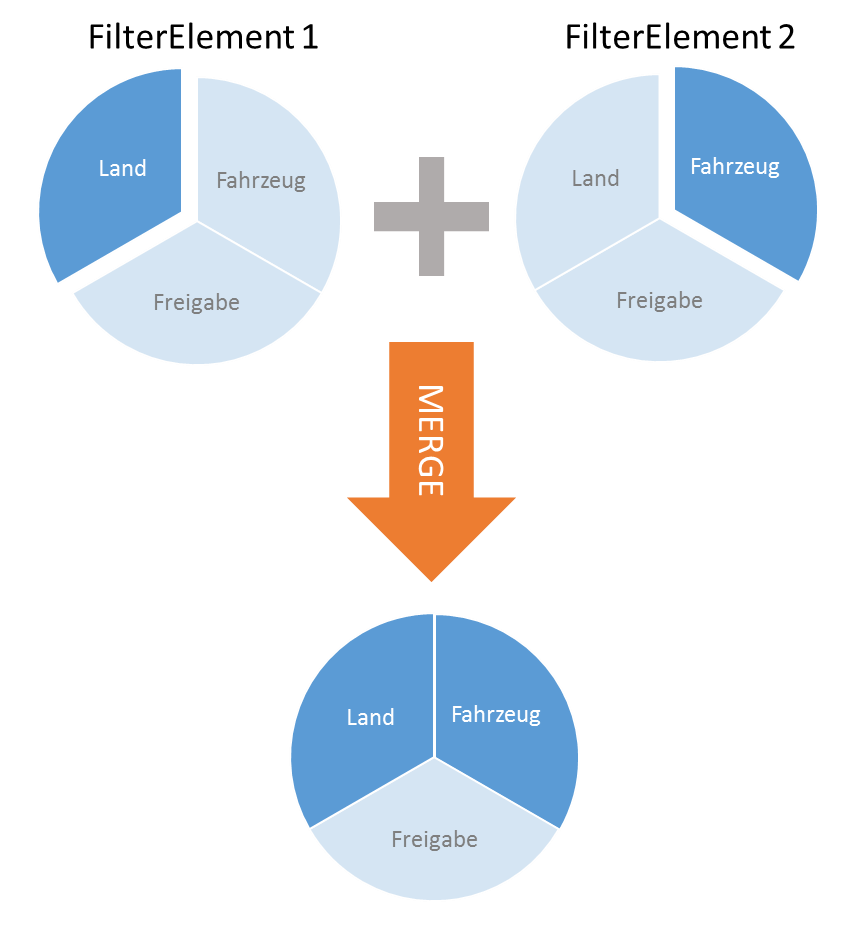
\includegraphics[width=0.65\textwidth]{grafiken/Multi_FilterElement.png}
 \caption{Schema FilterElement-Aufbau}
 \label{fig:multiFilter3}
\end{figure}

Ist der Vereinigungsvorgang nicht erfolgreich, weil zum Beispiel zwei Länder-Filter\-Ele\-men\-te übergeben wurden, wird eine \textit{IllegalArgumentException} geworfen.
Dieser Vorgang wird zur Erzeugung der \gls{ergebnismenge} für die Ergebnisansicht durchlaufen. Dies geschieht für jede mögliche Kombination der Elemente aus der Länder-\gls{ergebnismenge} mit den Elementen der Fahrzeugmenge. Es wird so das Kartesische Produkt (Abb. \ref{fig:multiFilter4}) der Mengen gebildet.

\begin{figure}[H]
 \centering
 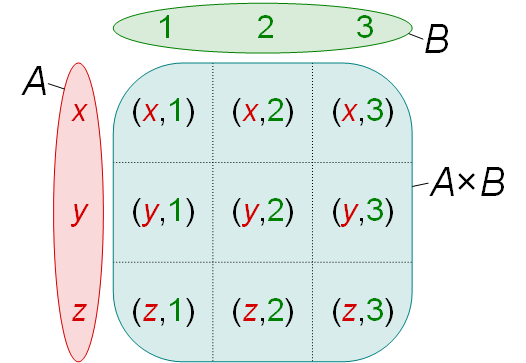
\includegraphics[width=0.4\textwidth]{grafiken/Multi_Kartesisches.png}
 \caption{Kartesisches Produkt}
 \label{fig:multiFilter4}
\end{figure}

Es ist leicht vorstellbar, dass die Elemente der \gls{ergebnismenge} und so auch die Anzahl ausgeführter Vereinigungen schnell anwachsen, wenn die Teilmengen größer werden. Die Komplexität dieses Programmteiles ist in der Groß-O-Notation $O(n^2)$. Es gibt aufgrund der Definition des Kartesischen Produktes keinen schnelleren Algorithmus. (Src) Daher muss die \textit{\#merge(FilterElement, FilterElement)}-Methode möglichst performant implementiert sein und nur ein Minimum an Instruktionen ausführen.

Der letzte Schritt, der für die Erzeugung der endgültigen Ergebnisdaten fehlt, ist das Laden und Setzen der \gls{freigabe}e. Anhand der erzeugten \gls{ergebnismenge} kann nun eine Datenbankabfrage durchgeführt werden, die nur eine eingeschränkte Anzahl an Freigabeobjekten lädt. Dazu wird das \gls{commandPattern} benutzt. Es wird also ein Command erzeugt und mit den Fahrzeug- und Länder-IDs an den Server gesendet. Der Server lädt die Freigabedaten daraufhin aus der Datenbank und schickt sie an den Client zurück. Die Ausführung des Commands und das Warten auf die Server-Antwort geschehen in einem anderen Thread als dem \gls{gui}-Thread, damit die Benutzeroberfläche nicht \enquote{einfriert}. Stattdessen kann während der Ladezeit ein Ladebalken, oder wie im Falle von \gls{falkofx}, eine benutzerdefinierte Ladeanimation angezeigt werden.

\section{Tabellenansicht} \label{sec:implTabelle}
\textbf{Problemstellung}

Die nächste zu bewältigende Anforderung ist die Ergebnispräsentation. Diese soll in einem ersten Schritt als Tabelle erfolgen. An der linken Seite befinden sich als Zeilendeklarator die Fahrzeuge. Für die Spaltenköpfe sind die Länder vorgesehen. Im Inhaltsbereich werden die zu Spalten- und Zeilendeklarator passenden \gls{freigabe}e angezeigt. 

\textbf{Konzept}

Die einzelnen Bildschirme werden bereits über eine zentrale Klasse geladen. Damit ein Bildschirm geladen werden kann, muss eine Klasse das Interface \textit{IScreen} implementieren. Es stellt die Methoden \textit{\#getContent()} und \textit{\#initialized()} zur Verfügung. Die erste Methode dient dem Zugriff auf ein UI-Objekt, das in den \gls{javafx}-Szenegraphen eingehängt wird und den Content-Bereich der Anwendung füllt. Unter diesem \gls{javafx}-\textit{Node} können weitere Knoten hängen, die den Aufbau einer komplizierten Benutzeroberfläche ermöglichen. Die zweite Methode dient als Callback und wird ausgeführt, sobald die Benutzeroberfläche initialisiert und angezeigt wurde. In dieser Methode können Aktionen ausprogrammiert werden, die erst nach Anzeige des UIs möglich sind (z.B. das Setzen von Daten in eine Tabelle oder das automatische Selektieren einer Zeile).

\begin{figure}[H] 
	\centering
	\subfloat[Schräge Spaltenköpfe] {
		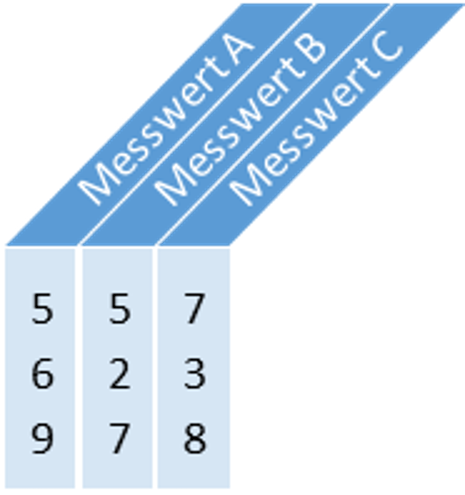
\includegraphics[width=0.25\textwidth]{grafiken/Tabelle_Inclined.png}
	}
	\hspace{2.0em}
	\subfloat[Normale Tabelle] {
		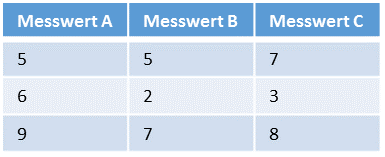
\includegraphics[width=0.5\textwidth]{grafiken/Tabelle_normal.png}
	}
	\caption{Vergleich: Schräge Spaltenköpfe - Normale Tabelle}
	\label{fig:tabelle1}
\end{figure}



Für die Benutzeroberfläche kann eine bereits bestehende Komponente angepasst verwendet werden. Bei der Komponente handelt es sich um eine \gls{javafx}-\textit{TableView}, die für das \gls{falkofx}-Projekt modifiziert wurde. Eine Besonderheit dieser Tabelle ist, dass sie über schräge Spaltenköpfe verfügt. Dies ist deshalb sinnvoll, damit sich die Spaltenbreite nicht an der Länge des Textes im Spaltenkopf orientieren muss, sondern nur an dem Inhalt der Zellen. Wenn man zuvor weiß, dass es Zellen gibt, die nur sehr kurze Inhalte haben (z.B. ein Icon oder eine kurze Zahl), kann man durch die Verwendung von schrägen Spaltenköpfen den verlorenen Platz minimieren.

Wie man anhand der Abbildung \ref{fig:tabelle1} erkennen kann, nimmt zwar die Höhe der Tabelle zu, die Breite wird jedoch viel effektiver ausgenutzt. Der Platz, der am rechten Rand durch die schrägen Spaltenköpfe entsteht, ist bei einer höheren Spaltenanzahl vernachlässigbar gering.

Ein weiterer Vorteil der Tabelle ist die mögliche Gruppierung von Spalten. Diese werden visuell von anderen Gruppen abgetrennt und bilden dementsprechend eine geschlossene Einheit (Abb. \ref{fig:tabelle2}).

\begin{figure}[H]
 \centering
 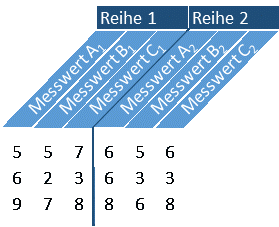
\includegraphics[width=0.5\textwidth]{grafiken/Tabelle_Grouped.png}
 \caption{Schräge Spaltenköpfe mit Gruppierung}
 \label{fig:tabelle2}
\end{figure}

Die Tabelle unterstützt außerdem das ein- und ausblenden von Spaltengruppen, sowie die Umsortierung dieser. In der Anwendung ist diese Funktion in der Seitenleiste untergebracht.

Die eigentlichen Informationen, die in der Ergebnisansicht präsentiert werden sollen, sind die Freigabedaten für die Fahrzeugproduktion. Um diese Daten zuordnen zu können, muss Im Spaltenkopf das Land angezeigt werden und am Anfang der Zeile das Fahrzeug mit ausgewählten technischen Daten. Die Informationen zu den technischen Daten sind notwendig, da zu einem Fahrzeug mehrere verschiedene Varianten existieren, die sich in mindestens einem Kriterium unterscheiden. Für jedes dieser Fahrzeuge ist die Freigabe eine andere. 

Wie bereits erwähnt (Abschnitt \ref{sec:implDataProvider}), sind die Hauptinformationen, die man aus einem \gls{freigabe} erhalten kann, das Start- und das Enddatum der Produktion. Daher ist es sinnvoll, diese beiden Daten auf den ersten Blick anzuzeigen. Dies geschieht, wie auch im Originalclient, durch die Angabe von Kalenderwoche und Jahr nach dem Schema \enquote{KW/YY}. Daher ist das folgende Layout denkbar:

\begin{figure}[H]
 \centering
 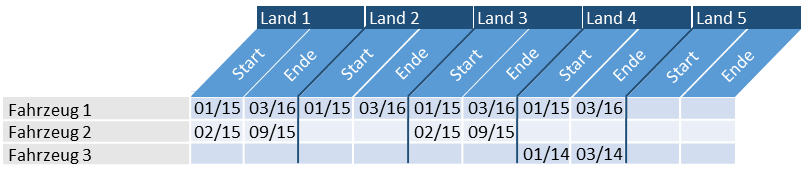
\includegraphics[width=1.0\textwidth]{grafiken/Tabelle_complete.png}
 \caption{Design Ergebnistabelle}
 \label{fig:tabelle3}
\end{figure}

\textbf{Umsetzung}

Die Umsetzung erfordert zunächst die geeignete Benutzeroberfläche. Ein Teil der Implementierungsarbeit ist bereits durch die vorhergegangenen Anwendungsfälle absolviert worden. Auch hier gibt es in beiden Fällen eine Tabellenansicht zur ganzheitlichen Darstellung der \gls{ergebnismenge}. Dazu gibt es bislang eine mit Generics parametrisierte Klasse, welche die Ergebnisdarstellung verwaltet. So kann die Darstellung für das erste und das zweite Szenario ohne Änderungen an der Klasse genutzt werden. Auch wenn die Tabelle des dritten Anwendungsfalles denen der anderen beiden vom Aussehen stark ähnelt, kann der bereits existierende Code diese Ansicht nicht erzeugen.

Die bisherige Darstellung ist darauf ausgelegt, dass in jeder Zeile genau ein Modelobjekt mit all seinen Attributwerten angezeigt werden soll. Dabei sind die Spalten mit den entsprechenden Attributnamen betitelt. Die Problematik die hier vorliegt ist jedoch eine andere. Für den Fahrzeugbereich, der in Abbildung \ref{fig:tabelle3} noch grau angezeigt wird, kann das bisherige Prinzip weiter verwendet werden. Es werden Fahrzeugname und einige weitere technische Details angezeigt, für die wiederum jeweils eigene Spalten mit schrägen Spaltenköpfen existieren (auf Abb. \ref{fig:tabelle3} nicht abgebildet). Es ist sinnvoll, dass dieser Bereich an die Ergebniskonfiguration der Seitenleiste gekoppelt ist, da man ggf. mal mehr, mal weniger Details zu den Fahrzeugen einsehen möchte. Für den Hauptbereich allerdings, in dem die Freigabedaten angezeigt werden, funktioniert das bisherige Prinzip nicht. Die Länder, welche die neuen Spaltengruppierungen bilden, sind keine \gls{attribut}e der dargestellten Modelobjekte, sondern Werte aus der Teilergebnismenge des \gls{filter}s (Länder-Subfilter), die sich als Teil der Freigabeobjekte wiederfinden.

Nun könnte man eine neue Ergebnisansicht erstellen, die genau dieses Problem behandelt, dann allerdings müsste noch die linke Seite der Tabelle erzeugt werden – die Seite mit den Fahrzeugdaten. Um doppelten Code zu vermeiden, bietet sich hier die Möglichkeit an, die Klasse für die Ergebnisansicht zu abstrahieren und eine generische Klasse für den ersten und zweiten Anwendungsfall davon abzuleiten, sowie eine spezifische Klasse für den 3. Anwendungsfall.

Die \gls{javafx} \textit{TableView} lässt pro Tabelle nur eine Art von Modellobjekten zu. Diese Objekte stellen dann immer genau eine Zeile dar. Die Werte für die einzelnen Zellen werden mit Hilfe eines \textit{CellValueResolvers} bestimmt, der pro Tabellenspalte gesetzt wird und so den Wert an einem Schnittpunkt von Tabellenzeile und -spalte bestimmen kann - folglich den Wert einer Zelle. Für die Implementierung bedeutet das, die zusammengesetzten \gls{filterElement}e können nicht direkt aus der \gls{ergebnismenge} in die Tabelle gesetzt werden, sondern müssen gruppiert und für jede Zeile in einem Objekt zusammengefasst werden. Zu diesem Zweck wird die neue Datenstruktur \textit{FreigabeLineObject} eingeführt, die eine beliebige Anzahl an \textit{\gls{freigabe}n} enthält, eine Schnittstelle, um auf diese zuzugreifen, sowie eine Möglichkeit das Fahrzeug zu erhalten, nach dem die Werte gruppiert wurden. Aus technischer Sicht wurde die Datenstruktur auf Basis einer \textit{HashMap} aufgebaut, welche mit Hilfe ID als \textit{Key} den Zugriff darauf erlaubt. Die Werte der \textit{HashMap} entsprechen den \gls{filterElement}en, welche jeweils ein spezifisches \gls{freigabe} enthalten.

Das Problem, das nun auftritt, ist, dass die Tabellen auf den Modellobjekten (in dem Fall \gls{filterElement}e) basieren, es sollen jedoch Elemente vom Typ FreigabeLineObject dargestellt werden. Um dieses Konzept in die vorgestellte Klassenstruktur zu integrieren, muss der \textit{AbstractResultTableController} mit 2 generischen Parametern versehen werden (Abb. \ref{fig:tabelle4}). Der erste Parameter steht für den Typ der Modelelemente, auf denen die Ansicht basiert, der zweite Parameter bestimmt den Typen der Zeilenobjekte, die in der Ergebnistabelle landen. Die Unterklassen spezifizieren diese Parameter daraufhin genauer. Es werden außerdem Methoden benötigt, um aus der \gls{ergebnismenge} der Modelobjekte die Zielergebnismenge zu generieren und umgekehrt aus einem Zeilenobjekt ein spezifisches Modelobjekt zu erhalten.

Die generische Klasse \textit{GenericResultTableController} löst das Problem so, dass sie nur noch einen Parameter (\textit{T}) besitzt, der sowohl für das \textit{T} als auch das \textit{R} der Oberklasse steht. Auf diese Weise sind die Modellobjekte gleich den Objekten, die in der Ergebnistabelle pro Zeile angezeigt werden (Abb. \ref{fig:tabelle4}). Bei dem spezifischen \textit{FreigabeResultTableController} werden die Parameter mit den konkreten Klassen \gls{filterElement} und FreigabeLineObject überschrieben (Abbildung \ref{fig:tabelle4}).

\begin{figure}[H]
 \centering
 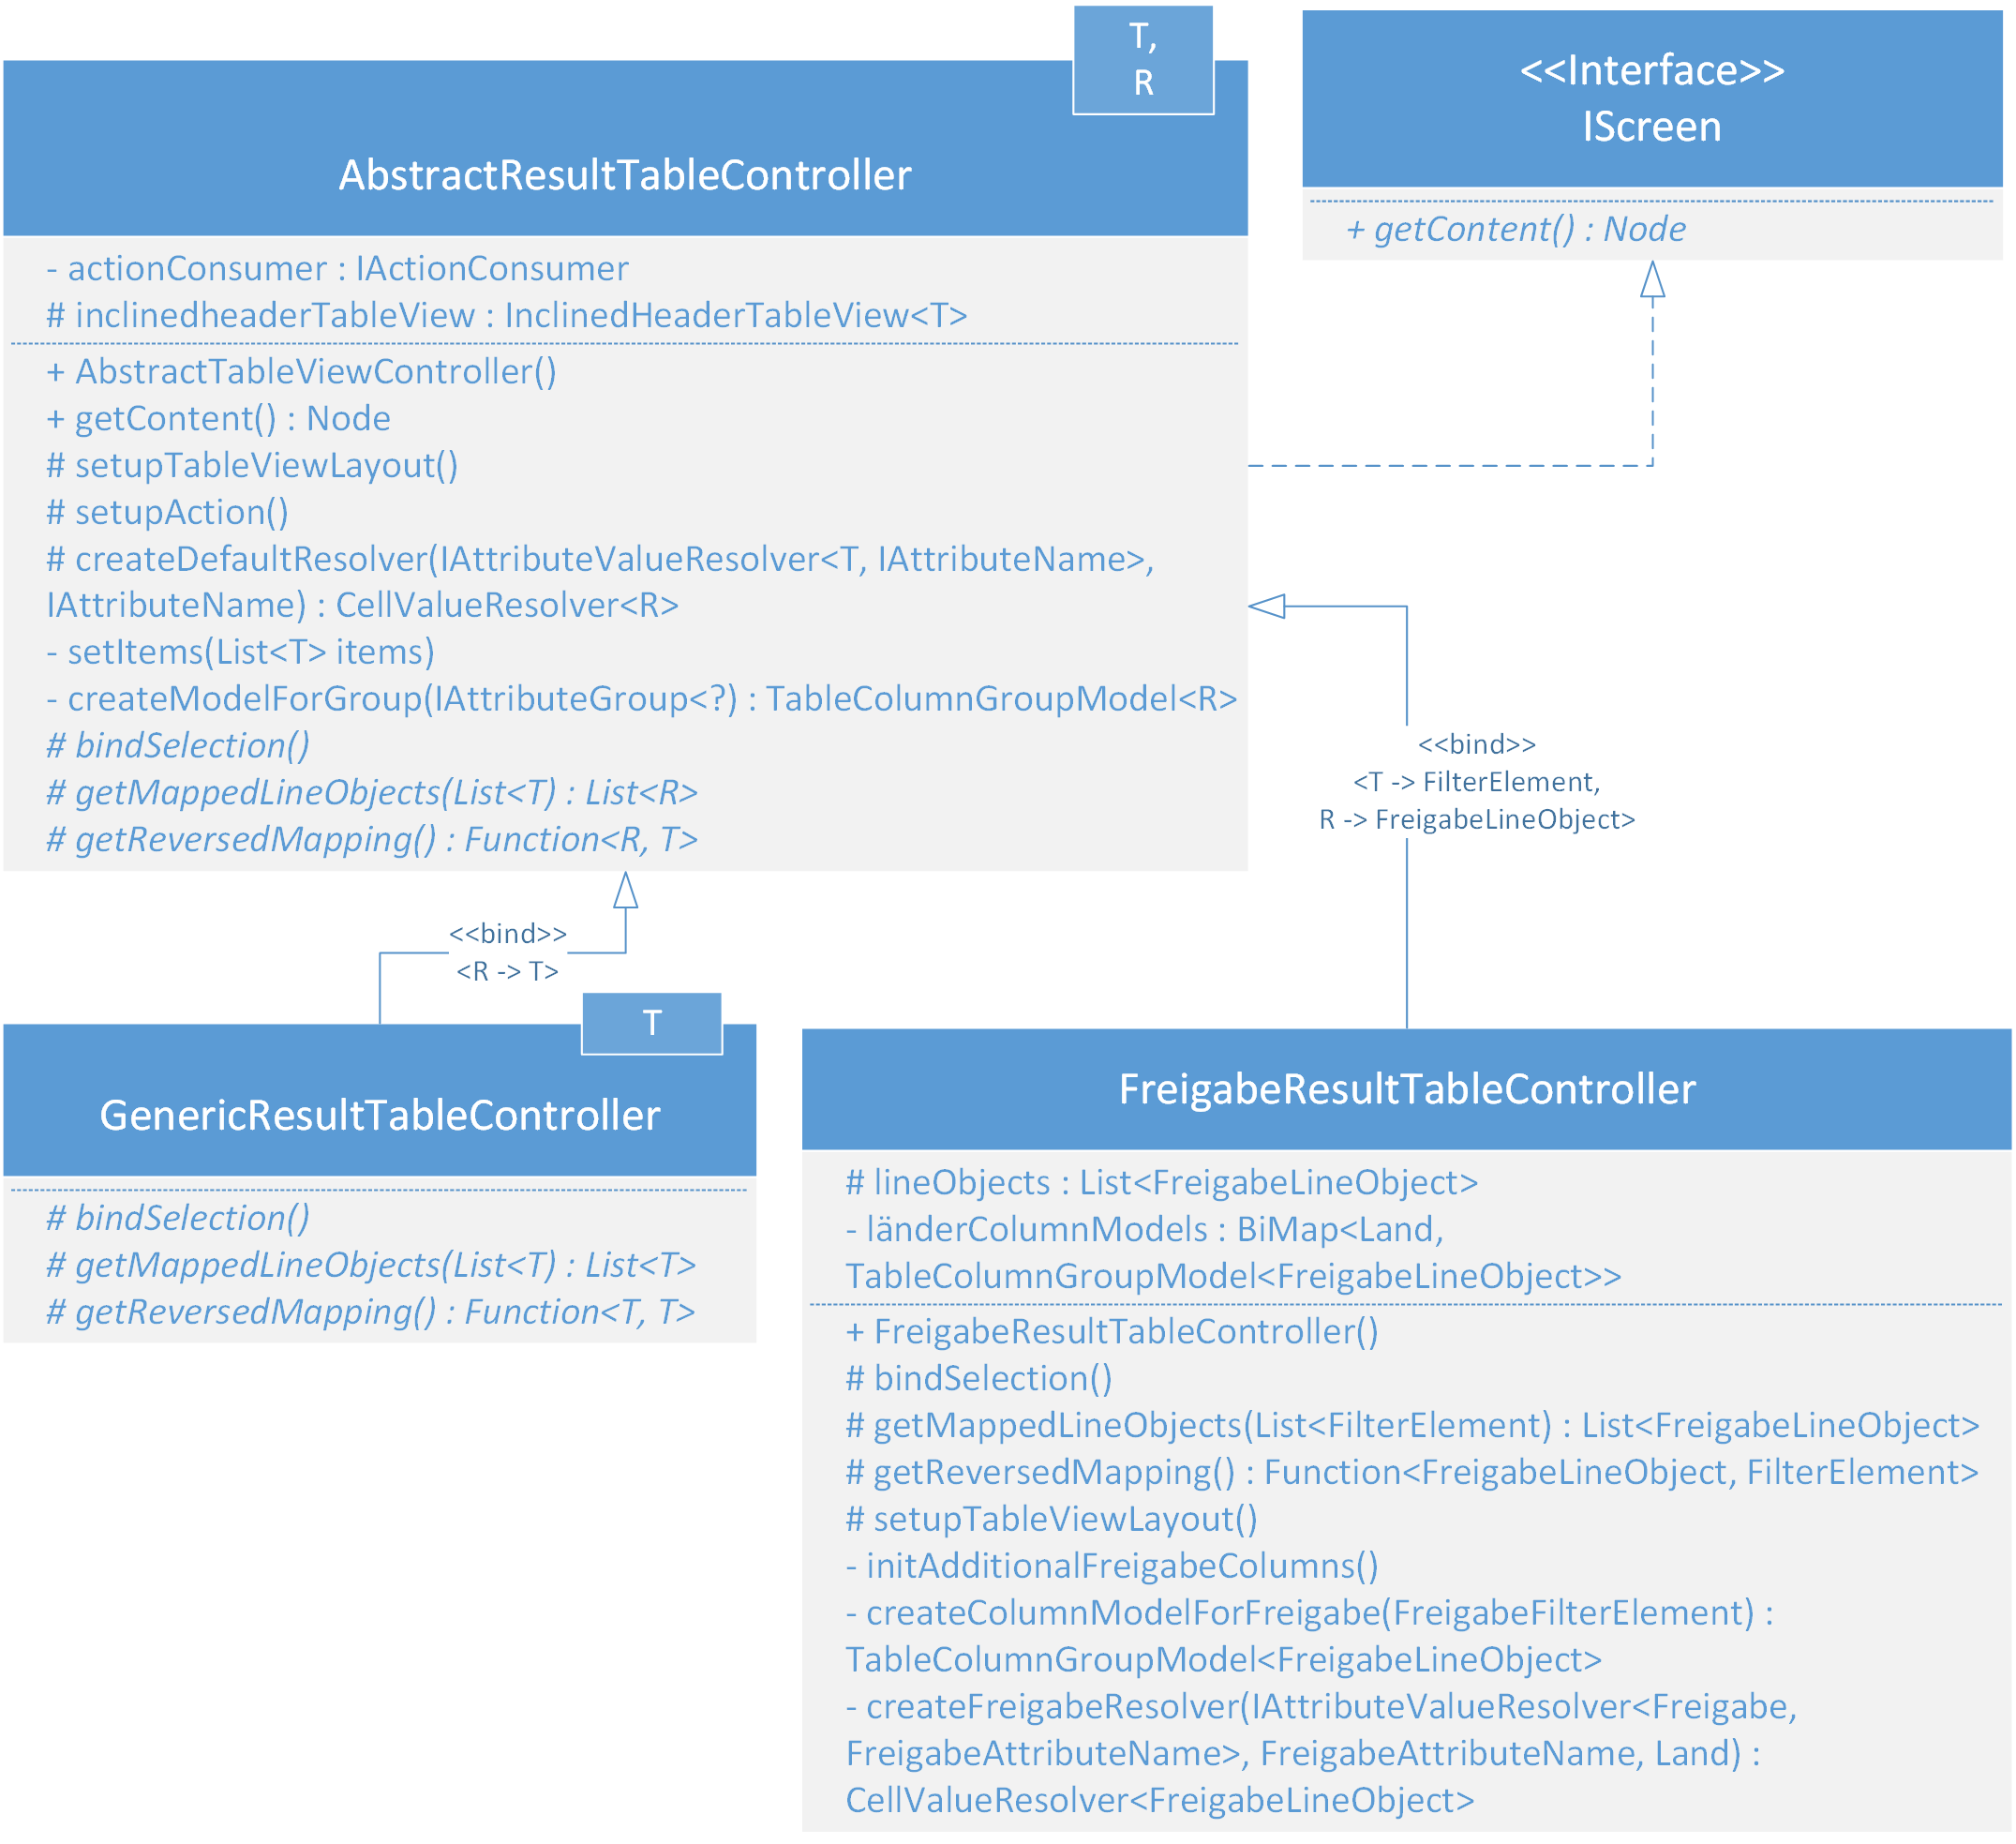
\includegraphics[width=1.0\textwidth]{grafiken/Class_ResultTable.png}
 \caption{Klassendiagramm Ergebnisansicht}
 \label{fig:tabelle4}
\end{figure}

Für die zu überschreibenden abstrakten Klassen ist die Implementierung des GenericResultTableControllers denkbar simpel.


\begin{lstlisting}[
    language=Java,
    caption=GenericResultTableController - Mapping-Methoden,
    label=code10]
	public List<T> getMappedLineObjects(List<T> data) {
		return data;
	}

	public Function<T, T> getReversedMapping() {
		return Function.identity();
	}
\end{lstlisting}

Bei dem FreigabeResultController fällt die Umsetzung etwas komplizierter aus. Bereits beim Konstruktoraufruf werden die Modelobjekte der \gls{ergebnismenge} in die Zeilenobjekte \enquote{verpackt}. Zu diesem Zweck gibt es eine Membervariable vom Typ \textit{List<Frei\-ga\-be\-Line\-Ob\-ject>}. Diese Liste wird befüllt, indem für jedes Element aus der \gls{ergebnismenge} zunächst ein Zeilenobjekt erstellt wird, das dieses Element enthält. Daraufhin wird mit der \textit{List\#con\-tains(Ob\-ject o)}- Methode überprüft, ob dieses Element schon in der Liste vorhanden ist. Dafür wird die \textit{\#equals()}-Methode der Zeilenobjekte aufgerufen. Da diese überschrieben wurde, liefert sie genau dann \textit{true} zurück, wenn die ID des zugeordneten Fahrzeuges bei beiden Zeilenobjekten gleich ist. Ist das der Fall, kann das überprüfte \gls{filterElement} dem bestehenden hinzugefügt werden, andernfalls wird das erzeugte FreigabeLineObject in die Liste der Zeilenobjekte eingegliedert. Die \#getMappedLineObjects()-Methode kann diese Liste nun sortiert zurückgeben.

Der Vorteil daran, dass die Liste schon zuvor beim Konstruktoraufruf erzeugt wird, und nicht erst bei Bedarf, ist der, dass die Benutzeroberfläche nicht \enquote{einfriert}. Die Methode \textit{\#getMappedLineObjects()} wird nach dem Aufbauen der Benutzeroberfläche im \gls{gui}-Thread ausgeführt. Wenn die Liste schon vorher erzeugt wurde, fällt an dieser Stelle der Großteil des Rechenaufwandes weg und der Aufbau der Oberfläche erscheint flüssiger.

Während der Konstruktionsphase werden, neben dem Tabellenlayout für die Spalten der Fahrzeugattribute, auch die zusätzlichen Freigabe-Spalten erzeugt, die nach Ländern gruppiert sind und das Start- und Enddatum als konkrete Spalten aufweisen. Auch hier werden wieder die Ergebnisdaten benötigt.

Als erster Schritt wird eine \textit{Map} erzeugt, die für jedes Land aus der \gls{ergebnismenge} ein \textit{ColumnGroupModel} verwaltet. Als technische Ausprägung dieser Map wird eine \textit{HashBiMap} aus der \textit{Google Guava} Library verwendet. Die Besonderheit und der Zweck dieser Datenstruktur werden später erläutert. Durch Java 8– Features kann der grundlegende Code für die Erzeugung der \textit{Map} relativ gering gehalten werden.

\begin{lstlisting}[
    language=Java,
    caption=Erzeugung der BiMap,
    label=code11]
	countryColumnModels = HashBiMap.create(
			ucContext.getResultData().stream()
			.collect(Collectors.toMap(
					freigabe -> freigabe.getLand(),	// Erzeugung des Keys
					this::createColumnModelForFreigabe, // Erzeugung des Wertes
					(o1, o2) -> o1	// Merge-Function, falls 2 Keys gleich
	 		))
	);
\end{lstlisting}

Die Methode \textit{\#createColumnModelForFreigabe() }erstellt auf Basis eines beliebigen \gls{filterElement}s eine Spaltengruppe mit den beiden Spalten für das Start- und Enddatum der Produktionsfreigabe. Dazu gehört ein \textit{CellValueResolver}, der für eine Zelle dieser Spalte anhand des darunterliegenden Zeilenobjektes den Wert dieser Zelle bestimmen kann. Beim Erstellen des CellValueResolvers wird die Länderinformation aus dem \gls{filterElement} übergeben. Anhand der Länder-ID kann dann der richtige Wert für eine Zelle aus dem Zeilenobjekt ermittelt werden. Schlussendlich müssen die Spaltengruppen aus der Map nur noch sortiert werden und der angepassten TableView hinzugefügt werden.

In Abbildung \ref{fig:tabelle4} wird ersichtlich, dass der FreigabeResultTableController über eine weitere Methode verfügt, die hier von Relevanz ist – die \textit{\#bindSelection()}-Methode. Diese sorgt dafür, dass das selektierte Modelobjekt, das global (im sogenannten \textit{Context}) verfügbar ist, aktuell gehalten wird. An diese Selektion ist beispielsweise die Sidebar gebunden, in der es eine Ergebnisvorschau gibt, die das derzeit angewählte Element farblich differenziert darstellt. Um dies in der komplexen Tabelle des 3. Anwendungsfalles zu ermöglichen, wird an die \gls{javafx}-Property der selektierten Zellen ein Listener angehängt. Darin wird die \textit{TablePosition} der Selektion bestimmt, durch welche die Spalte bestimmt werden kann, in der die Selektion stattgefunden hat. Problematisch ist es jetzt jedoch, das eigentliche Modellobjekt (vom Typ \gls{filterElement}) zu identifizieren, da über die Selektion nur das Zeilenobjekt erhalten werden kann. Zur Erinnerung: Um von einem FreigabeLineObject auf ein \gls{filterElement} schließen zu können, wird das Länderobjekt benötigt. An dieser Stelle kommt die zuvor erwähnte HashBiMap ins Spiel. Diese hat nämlich die Eigenheit, dass sowohl die Keys als auch die Values eindeutig zu identifizieren sind. Es entsteht also eine eineindeutige Beziehung zwischen den Objekten. Aus diesem Grund lassen sich die eigentlichen Values auch als Keys verwenden. Durch den Aufruf \textit{\#inverse()} auf der \textit{BiMap} wird diese invertiert und die vorherigen Keys werden zu Values und umgekehrt. Durch die zuvor ermittelte Spalte kann das dazugehörige Spaltengruppenmodell identifiziert werden und dadurch das zugehörige Land (aus der invertierten BiMap). Mit Hilfe des Landes lässt sich nun auf das Modellobjekt schließen, das daraufhin im Context aktualisiert wird.

Die letzte verbliebene Methode ist \textit{\#setupAction()}. Der Zweck dieser Methode ist das Ermöglichen von Interaktionen mit der Tabelle. Zum Beispiel kann bei einem Doppelklick eine Detailansicht zu einem selektierten Modellobjekt angezeigt werden.

Zur größeren Übersichtlichkeit bei der Navigation durch die umfangreiche Tabelle, wird neben der Zelle, die derzeit selektiert ist, auch die Spalte in einem helleren Farbton mit eingefärbt. So lässt sich schnell das zu einer Freigabe gehörende Fahrzeug identifizieren. Aufgrund der Tatsache, dass eine \gls{javafx} TableView nur entweder Reihenselektion oder Zellselektion nativ unterstützt, musste eine andere Lösung für das Hervorheben gefunden werden. Diese bestand in dem Setzen einer selbst definierten \gls{css}-Pseudoklasse, die genau dann auf eine Zeile angewandt wird, wenn Zellselektion aktiviert ist und eine Zelle aus der betroffenen Zeile selektiert wurde. Andernfalls würden die Standard-\gls{css}-Definitionen für Tabellenzeilen angewandt werden.